\quad \quad This subsystem communicates and controls database and Graphical user 
interface. This is needed for setting up the initial database for all the users, 
admin, students, etc. 

\begin{figure}[h!]
	\centering
 	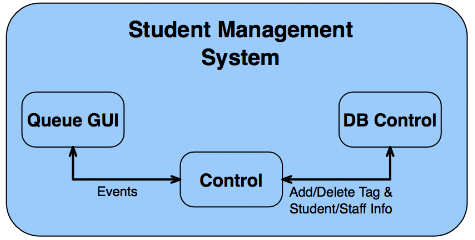
\includegraphics[width=0.60\textwidth]{images/ads_3}
 \caption{Student Management Subsystems}
\end{figure}

\subsection{Queue GUI Subsystem}
\quad \quad This subsystem will talk with the control subsystem and displays the list of the 
names of students in the GUI.

\subsubsection{Assumptions}
\quad \quad The GUI has to be running at the same time and the database must have the data of 
the students who are assigned a RFID tag.

\subsubsection{Responsibilities}
\quad \quad This subsystem accepts mouse and keyboard inputs from the user and update the list 
accordingly.

\subsubsection{Subsystem Interfaces}
\quad \quad This system has two, two-way interfaces. The first is directly connected to the 
computer recieving keyboard and mouse input and relaying to the screen. The second 
passes and receives from Control.

\begin {table}[H]
\caption{Student Management Queue GUI Subsystem interfaces} 
\begin{center}
    \begin{tabular}{ | p{1cm} | p{6cm} | p{3cm} | p{3cm} |}
    \hline
    ID & Description & Inputs & Outputs \\ \hline
    \#01 & GUI Interaction & \pbox{3cm}{User Input} & \pbox{3cm}{Events}  \\ \hline
    \#02 & Events Return & \pbox{3cm}{GUI Data} & \pbox{3cm}{Screen Data}  \\ \hline
    \end{tabular}
\end{center}
\end{table}

\subsection{Control Subsystem}
\quad \quad This subsystem communicates with the database subsystem and the queue display 
subsystem and vice versa. It also reformats the data.

\subsubsection{Assumptions}
\quad \quad There has to be working input systems to get the user input and a database and GUI 
to handle the events.

\subsubsection{Responsibilities}
\quad \quad This subsystem handles the callback functions. It should act as a control unit 
between the GUI and the database. It also checks for the safe use for security.

\subsubsection{Subsystem Interfaces}
\quad \quad This system has two, two-way interfaces. The first is connected to the Queue GUI 
recieving GUI events and returning data to the GUI. The second 
passes and receives from DB Control.

\begin {table}[H]
\caption {Student Management Control Subsystem Interfaces} 
\begin{center}
    \begin{tabular}{ | p{1cm} | p{5cm} | p{4cm} | p{3cm} |}
    \hline
    ID & Description & Inputs & Outputs \\ \hline
    \#03 & Control GUI & \pbox{4cm}{Events} & \pbox{3cm}{Database Query}  \\ \hline
    \#04 & Control Database & \pbox{4cm}{Database Response} & \pbox{3cm}{QUI Data}  \\ \hline
    \end{tabular}
\end{center}
\end{table}

\subsection{DB Control Subsystem}
\quad \quad This subsystem handles all the data related to students needing to be dismissed by 
staff. This is the subsystem that handles forwarding and receiving information from 
the database.

\subsubsection{Assumptions}
\quad \quad All the data has been set up in the database and it should be receiving good data 
from the control sub system.

\subsubsection{Responsibilities}
\quad \quad This subsystem will return all the data requested by the Control subsystem querying the DB.

\subsubsection{Subsystem Interfaces}
\quad \quad This system has two, two-way interfaces. The first is connected to the database, 
sending queries and receiving responses.  The second passes and receives from Control.

\begin {table}[H]
\caption {Student Management DB Control Subsystem interfaces} 
\begin{center}
    \begin{tabular}{ | p{1cm} | p{4cm} | p{4cm} | p{4cm} |}
    \hline
    ID & Description & Inputs & Outputs \\ \hline
    \#05 & Send Query & \pbox{4cm}{Database Query} & \pbox{4cm}{Query}  \\ \hline
    \#06 & Receive Results & \pbox{4cm}{Response} & \pbox{4cm}{Database Response}  \\ \hline
    \end{tabular}
\end{center}
\end{table}
